\chapter{Indledning}
\vspace*{0.5 cm}
\emph{Musik er en naturlig del af hverdagen. 
	Om det er baggrundsmusikken nede i Brugsen, en Grøn Koncert eller i høretelefonerne i bussen, er den altid til stede. 
	At musikken er så væsentlig en størrelse giver anledning til at undersøge hvilke optimeringsmåder man kan foretage sig, for at få den bedst mulige oplevelse ud af det - hver især. 
	En equalizers egenskab er at forme en musikafspillers lydsignal, så musikken lyder som brugeren finder bedst. 
	I denne rapport vil læseren blive guidet gennem processen bag ved udvikling af en digital equalizer - fra musikafspillerens udgangssignal til det ønskede lydsignal.}

\section{Formål}
%\note{Indledningen skal ikke handle om rapporten, men om rapportens emne. Man kan sige, at den kridter banen op ved at præsentere emneområdet.
%	\\
%	* Hvilket overordnet emne tager rapporten udgangspunkt i? \\
%	* Hvilket specifikt problem vil man derfor tage fat i og kigge nærmere på? }
%
%Formålet med projektet er, at forene de opnåede fagligheder fra undervisningen, samt at træne den studerende i, at kunne forstå og forklare afgrænsede systemer med funktionalitet der relaterer til faglighederne i Indlejrede Systemer og Signalbehandling, på 4. semester Elektronik og Datateknik. Fagene fra semesteret der indgår i projektet er Embedded programmering, Analoge filtre og signaler og Operativsystemer. Ledningsteori som er et mindre fag under Analoge filtre, er ikke med i rapporten, da undervisningen ligger så sent i semesteret, at der ikke er tid til at se på implementation af faget i rapporten.
%
%Semesterets fagbeskrivelse vil blive brugt som tjekliste, for at komme igennem så meget af stoffet som muligt.
Formålet med dette projekt, er at formidle de opnåede fagligheder fra 4. semesters undervisning på uddannelsen diplomingeniør i elektronik og datateknik. Semesterets hovedemne omhandler "Indlejrede systemer og signalbehandling", hvor fagene "Analoge filtre og signaler", "Digital signalbehandling", "Embedded programmering" og "Operativsystemer" er inkluderet. Der skal på et grundlæggende niveau, kunne relateres til faglighederne i ét samlet produkt ud fra disse. For at kunne håndtere dette, vil semesterets fagbeskrivelse blive anvendt til at opnå det ønskede formål.


\section{Problemformulering}
%\note{Generel fortælling om hvordan man kan finde frem til en projekt der kan blive dækket af de fagligheder de skal omhandle}
%
%\note{Specefike problemer der kan være ved at lave en equalzier som et embedded system}
%
%\note{Hvilke spørgsmål kan der stilles om man ønsker at få besvaret ?}

%Ud fra formålet med projektet, er der blevet valgt, at udvikle en digital equalizer, da den dækker centrale punkter af fagbeskrivelsen. De væsentligste punkter som projektet dækker er analog og digital filterteori, signalbehandling og strukturelle opbygning af et operativ system.

%\note{Problemformulering: Hvilket spørgsmål vil denne rapport helt præcist stille skarpt på, og hvilke delspørgsmål vil det måske være nødvendigt at besvare for at kunne besvare hovedspørgsmålet?}
%
%Hovedspørgsmålet som der vil blive fokuseret på er:
%\begin{enumerate}
%	\item Hvilken digital signalbehandling kan give den ønskede signal filtrering?
%\end{enumerate}
%Herunder ses underspørgsmålene som vil blive brugt til at besvare hovedspørgsmålet:
%\begin{enumerate}
%	\item Kan en digital equalizer realiseres ved hjælp af en Tiva™ TM4C123GH6PM Microcontroller?
%	\item Kan EMP boarded fra Embedded Programmering anvendes i projektet?
%	\item 
%\end{enumerate}
%\note{
%Projektet går ud på at designe en parametrisk equalizer, der kan efterbehandle et lydsignal. Den skal realiseres ved hjælp af en Tiva™ TM4C123GH6PM Microcontroller som er platformen i faget Embedded Programmering. Equalizeren skal have nogle forudbestemte bånd, og samtidig have et bånd som brugeren frit kan modulere.
%}
Ud fra formålet for projektet, er der blevet valgt at fremstille et produkt, hvori alle fagligheder kan anvendes. 
Produktet der ønskes realiseret, er konstruktionen af en digital parametrisk\footnote{Uddybende forklaring om forskellen mellem parametrisk og grafisk equalizer sker i kapitel \ref{kap:equalizer}.} equalizer. 
Denne parametriske equalizer, skal realiseres ved en mikrocontroller af samme type, der anvendes som platformen i faget embedded programmering.
Equalizeren skal have nogle såkaldte "bånd" med justerbarer parametre, som fx frekvens og forstærkning. 
Ud fra fagbeskrivelsen, kan dette relateres i et så bredt omfang, at formålet opfyldes. 
Problemformuleringen forlyder sig derfor som følgende: \\

En digital parametrisk equalizer ønskes realiseret ved en mikrocontroller hvor der anvendes digital signalbehandling og analog filterteori. 
Herunder ønskes en brugerflade, som interagerer med systemet. 
Denne brugerflade skal kunne håndtere equalizerserens båndprofiler.\\

Der ønskes herudover svar på følgende problemstillinger:
\begin{itemize}[noitemsep]
	\item Hvilke digitale signalbehandlingsmetoder er bedst til fremstilling af en digital equalizer?
	\item Hvordan kan et analogt filter anvendes på en digital equalizer?
	\item Hvordan anvendes digital signalbehandling, til at give de ønskede båndspecifikationer?
	\item Hvilke krav er der til de analoge filtre i forhold til den samlede signalbehandling.
	\item Hvordan fremstilles og designes software der kan håndtere digital sampling og gengivelse af lydsignalet
\end{itemize}

\section{Projektafgrænsning}
%\note{Hvilke emner / delemner kommer rapporten ikke ind på? Hvorfor?\\
	%Det er meget almindeligt, at problemformulering og metoderedegørelse simpelthen er en del af indledningen, men så bør de normalt være markeret med underrubrikker (under-overskrifter) for overskuelighedens skyld. Hvis du er uddannelsessøgende, så tjek, om skolen eller institutionen (eller din vejleder) har særlige krav på det punkt.}

En equalizer kan realiseres både analogt og digitalt.
I projektet vil den blive realiseret digitalt, da faget embedded programmering skal indgå. 
Der træffes endvidere valget om at gøre den parametrisk, for bedre fleksibilitet. 
Følgende medtages ikke i rapporten og afgrænser projektet:
\begin{itemize}[noitemsep]
	\item Equalizeren bliver udviklet som prototype og ikke et produktionsklart produkt.
	\item Der vil blive lagt vægt på at eftervise funktionaliteten af signalbehandlingen og ikke hvor god lydkvalitet det endelige produkt lever op til.
	\item Koden som er anvendt til equalizeren, er så vidt muligt af eget design. Enkelte steder er kode fra 3. part anvendt, herunder moduler og kode eksempler fra undervisningen.
\end{itemize}

\section{Kravspecifikation} \label{afs:kravspecifikation}
I dette afsnit fremstår de opsatte krav for projektet.
Disse er fastsat dels ud fra kravet til selve projektbeskrivelsen og dels for at efterligne den virkelige ingeniørverden.

\begin{itemize}[noitemsep]
	\item Prototypen udvikles på Tiva™ C Series TM4C123G LaunchPad Evaluation Kit \cite{spmt281a}.
	\item Tiva™ TM4C123G serie Microcontroller anvendes \cite{spmu296}.
	\item Kildekoden er en del af produktet og skal overholde \textit{EMP C Code Standard}\cite{emp-c}.
	\item Equalizeren skal fungere som parametrisk equalizer.
	\item Det skal være muligt at ændre frekvensprofiler på equalizeren.
	\item Indgangs- og udgangssignaler skal overholde line-signal standard på, nominal $-10 dBV$, $0,894 V_{pp}$ (Forbruger elektronik line-signal).
	\item Tilgængelige filtertyper i frekvensprofiler - Highshelf, Lowshelf, Peek- og Notchfilter.
	\item Equalizerparametre skal omfatte - Frekvens, båndbredde og forstærkning.
	\item Equalizerens funktionalitet og effektivitet skal kunne efterprøves.
\end{itemize}


\section{Løsningsmodel}

\begin{figure}[h]
	\centering
	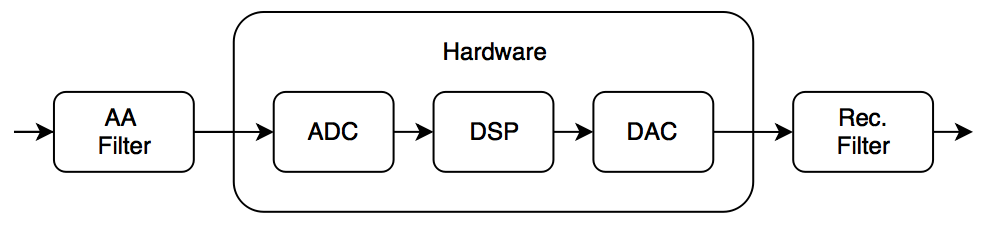
\includegraphics[width=0.8\linewidth]{billeder/flow_losn}
	\caption{Løsningsmodellen}
	\label{fig:losningsmodel}
\end{figure}

Løsningsmodellen som ses på figur \ref{fig:losningsmodel}, er delt op i tre hovedemner. Denne model gør det nemt at dele emnerne som indgår i rapporten op. Som første emne er der filtrene - altså både indgangs- og udgangsfiltret. Efter indgangsfiltret går man ind i hardware-blokken, som blandt andet indeholder den analoge til digitale konverter samt den digitale til analoge konverter. Til sidst er der emnet som indeholder den digitale signalbehandling, hvor de fs
\husk{Søren}{afsnit forklarer ikke modellen, og afsluttes noget hårdt}


\section{Proces- og arbejdsmetode}
%\note{Metodebeskrivelse: Hvordan vil det blive gjort? (Opgaven bygger på den-og-den litteratur samt interviews med dem og dem. Først undersøger vi dét, og så undersøger vi dét. Derefter …)}
Denne rapport er bygget op på baggrund af den faglige undervisning, hvor alle fag har spillet en væsentlig rolle. Dertilhørende litteratur er brugt til at studere nærmere specifikke omstændigheder, og ekspertviden er blevet hentet fra underviserne, med bedre forståelse for det faglige indhold. Der er arbejdet ud fra emneopdeling, hvor gruppen er blevet delt i 3, og har fået tildelt arbejdsopgaver ud fra dette. Der er så vidt muligt holdt statusmøder, hvor gruppen har diskuteret hver deres problemer. Der er derudover fulgt en overordnet tidsplan, hvor enkelte deadlines har været opretholdt. Der har været en del miskommunikation imellem gruppen igennem projektperioden, hvilket har gjort at tidsplan mm. har skredet. Der blev dog fundet en fornuftig løsning i samarbejde med gruppens vejleder.

\jj{Section skal rette lidt til, fyldeord skal fjernes}

%Gennemarbejdningen med denne rapport vil tage udgangspunkt i undervisningen med dertilhørende litteratur. Ekspertviden vil blive hentet fra underviserne, med henblik på bedre forståelse af stoffet. Rapporten er bygget op omkring signalvejen igennem equalizeren. Det kan derved lette forståelsen for, hvordan signalet ændres løbende igennem systemet.
%\husk{Kenneth}{Tage udgangspunkt i signalvejen - men bedre ord for det}


